\chapter{Rigid body dynamics solutions}
\begin{abox}
	Practice set 1 solutions
	\end{abox}
\begin{enumerate}
\begin{minipage}{\textwidth}
\item An annulus of mass $M$ made of a material of uniform density has inner and outer radii $a$ and $b$ respectively. Its principle moment of inertia along the axis of symmetry perpendicular to the plane of the annulus is:
	\exyear{NET DEC 2011}
\end{minipage}
\begin{tasks}(2)
	\task[\textbf{A.}] $\frac{1}{2} M \frac{\left(b^{4}+a^{4}\right)}{\left(b^{2}-a^{2}\right)}$
	\task[\textbf{B.}]$\frac{1}{2} M \pi\left(b^{2}-a^{2}\right)$
	\task[\textbf{C.}]$\frac{1}{2} M\left(b^{2}-a^{2}\right)$
	\task[\textbf{D.}]$\frac{1}{2} M\left(b^{2}+a^{2}\right)$
\end{tasks}
\begin{answer}
	The correct option is \textbf{(d)}
\end{answer}
\begin{minipage}{\textwidth}
	\item Two bodies of equal mass $m$ are connected by a massless rigid rod of length $l$ lying in the $x y$-plane with the centre of the rod at the origin. If this system is rotating about the $z$-axis with a frequency $\omega$, its angular momentum is
	\exyear{NET DEC 2012}
\end{minipage}
\begin{tasks}(2)
	\task[\textbf{A.}] $m l^{2} \omega / 4$
	\task[\textbf{B.}]$m l^{2} \omega / 2$
	\task[\textbf{C.}]$m l^{2} \omega$
	\task[\textbf{D.}]$2 m l^{2} \omega$
\end{tasks}
\begin{answer}
 \begin{align*}
 \text{Since rod is massless i.e}. M&=0.\\
 \text{Moment of inertia of the system} \quad I&=m_{1} r_{1}^{2}+m_{2} r_{2}^{2}, m_{1}=m_{2}=m \quad \text{and} \quad r_{1}=r_{2}=\frac{l}{2}\\
 I&=\frac{m l^{2}}{4}+\frac{m l^{2}}{4} \Rightarrow I=\frac{m l^{2}}{2}\\
 \text{Angular momentum,} \quad J&=I \omega \quad \text{and} \quad J=\frac{m l^{2} \omega}{2}
 \end{align*}
 The correct option is \textbf{(b)}
\end{answer}
\begin{minipage}{\textwidth}
	\item Two masses $m$ each, are placed at the points $(x, y)=(a, a)$ and $(-a,-a)$ and two masses, $2 m$ each, are placed at the points $(a,-a)$ and $(-a, a)$. The principal moments of inertia of the system are
	\exyear{NET DEC 2015}
\end{minipage}
\begin{tasks}(2)
	\task[\textbf{A.}] $2 m^{2}, 4 m a^{2}$
	\task[\textbf{B.}]$4 m a^{2}, 8 m a^{2}$
	\task[\textbf{C.}] $4 m a^{2}, 4 m a^{2}$
	\task[\textbf{D.}] $8 m a^{2}, 8 m a^{2}$
\end{tasks}
\begin{answer}
 \begin{align*}
 I_{x x}&=\sum_{i} m_{i}\left(y_{i}^{2}+z_{i}^{2}\right)=\sum m_{i} y_{i}^{2} \quad \because z_{i}=0\\
 \Rightarrow I_{x x}&=m a^{2}+m a^{2}+2 m a^{2}+2 m a^{2} \Rightarrow I_{x x}=6 m a^{2}\\
 \text{Similarly,} \quad I_{y y}&=6 m a^{2} \quad \text{and}\quad  I_{z z}=12 m a^{2}\\
 I_{x z}&=I_{z x}=0, I_{y z}=I_{z y}=0\\
 I_{x y}&=I_{y x}=-m_{i} \sum_{z} x_{i} y_{i}=-m\\
 I_{x y}&=I_{y x}=-m_{i} \sum_{i} x_{i} y_{i}=-m a^{2}-m a^{2}+2 m a^{2}+2 m a^{2} \Rightarrow I_{x y}=I_{y x}=2 m a^{2}
 \end{align*}
 Moment of inertia tensor
 $
 I=\left(\begin{array}{ccc}
 6 m a^{2} & 2 m a^{2} & 0 \\
 2 m a^{2} & 6 m a^{2} & 0 \\
 0 & 0 & 12 m a^{2}
 \end{array}\right)
 $	
 Eigen value of matrices is principal moment of inertia, which is given by
 $$
 \lambda_{1}=4 m a^{2}=I_{x}, \lambda_{2}=8 m a^{2}=I_{y}, \lambda_{3}=12 m a^{2}=I_{z}
 $$
 So, $I_{x}=4 m a^{2}$ and $I_{y}=8 m a^{2}$\\
 The correct option is \textbf{(b)}
\end{answer}
\begin{minipage}{\textwidth}
	\item A disc of mass $m$ is free to rotate in a plane parallel to the $x y$ plane with an angular velocity $-\omega \hat{z}$ about a massless rigid rod suspended from the roof of a stationary car (as shown in the figure below). The rod is free to orient itself along any direction.
	\begin{figure}[H]
		\centering
		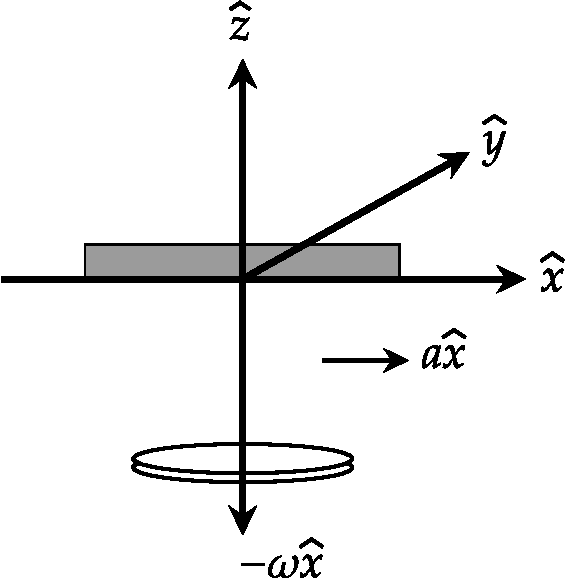
\includegraphics[height=4cm,width=5cm]{diagram-20210926(37)-crop}
	\end{figure}
	The car accelerates in the positive $x$-direction with an acceleration $a>0 .$ Which of the following statements is true for the coordinates of the centre of mass of the disc in the reference frame of the car?
	\exyear{NET DEC 2017}
\end{minipage}
\begin{tasks}(2)
	\task[\textbf{A.}] only the $x$ and the $z$ coordinates change
	\task[\textbf{B.}]only the $y$ and the $z$ coordinates change
	\task[\textbf{C.}]only the $x$ and the $y$ coordinates change
	\task[\textbf{D.}]all the three coordinates change
\end{tasks}
\begin{answer}
The correct option is \textbf{(d)}	
\end{answer}
\end{enumerate}
\newpage
\begin{abox}
	Practice set 2
	\end{abox}
\begin{enumerate}
\begin{minipage}{\textwidth}
	\item A uniform solid cylinder is released on a horizontal surface with speed $5 \mathrm{~m} / \mathrm{s}$ without any rotation (slipping without rolling). The cylinder eventually starts rolling without slipping. If the mass and radius of the cylinder are $10 \mathrm{gm}$ and $1 \mathrm{~cm}$ respectively, the final linear velocity of the cylinder is.............. $\mathrm{m} / \mathrm{s}$. (up to two decimal places).
	\exyear{GATE 2017}
\end{minipage}
\begin{answer}
$m v r=m v_{c m} r+I_{c m} \omega=m v_{c m} r+\frac{1}{2} m r^{2} \frac{v_{c m}}{r} \Rightarrow v=\frac{3}{2} v_{c m} \Rightarrow v_{c m}=\frac{2}{3} v=\frac{10}{3}=3.33 m / \mathrm{sec}$	
\end{answer}
\begin{minipage}{\textwidth}
	\item A uniform circular disc of mass $m$ and radius $R$ is rotating with angular speed $\omega$ about an axis passing through its centre and making an angle $\theta=30^{\circ}$ with the axis of the disc. If the kinetic energy of the disc is $\alpha m \omega^{2} R^{2}$, the value of $\alpha$ is (up to two decimal places).
	\exyear{GATE 2018}
	\begin{figure}[H]
		\centering
		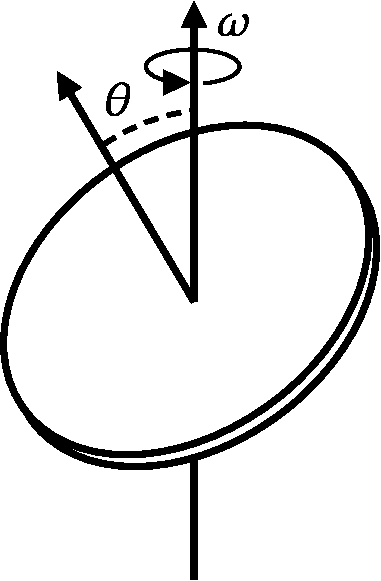
\includegraphics[height=3cm,width=3cm]{diagram-20210915(17)-crop}
	\end{figure}
\end{minipage}
\begin{answer}
\begin{align*}
\intertext{The kinetic energy of the disc is,}
T&=\frac{1}{2} \vec{L} \cdot \vec{\omega}
\intertext{Where $\vec{L}$ is angular momentum and $\omega$ is angular velocity}
T&=\frac{1}{2}|\vec{L}||\vec{\omega}| \cos 30^{\circ}=\frac{1}{2} I \omega \cdot \omega \frac{\sqrt{3}}{2}=\frac{1}{2}\left(\frac{m R^{2}}{2}\right) \omega^{2} \times \frac{\sqrt{3}}{2} \\
T&=\frac{\sqrt{3}}{8} m \omega^{2} R^{2}=0.21 m \omega^{2} R^{2} \Rightarrow \alpha m \omega^{2} R^{2}=0.21 m \omega^{2} R^{2}
\end{align*}
Hence, $\alpha=0.21$	
\end{answer}
\end{enumerate}